%\documentclass[12pt,a4paper]{report}	
%\input{Formatting_TEMPL8}
%
%% Make start at chapter 2
%\setcounter{chapter}{1}
%\begin{document}
	
% ===================
\chapter{Review of Related Literature and Studies}
	\lipsum[6]


\section{Digital Communications Systems}
	\lipsum[2-3]

	\begin{equation}
		x=\frac{b\pm\sqrt{b^2-4ac}}{2a}
		\label{eq:quadratic}
	\end{equation}
	
	Equation \ref{eq:quadratic} \lipsum[4]
	
	Additionally, this is a sample of in-line equation $2+2=5$
	
	
\subsection{Digital Modulation Schemes}
	\lipsum[7]
	
	\begin{figure}[htbp]
		\begin{adjustwidth}{1.25cm}{0pt}
			\centering
			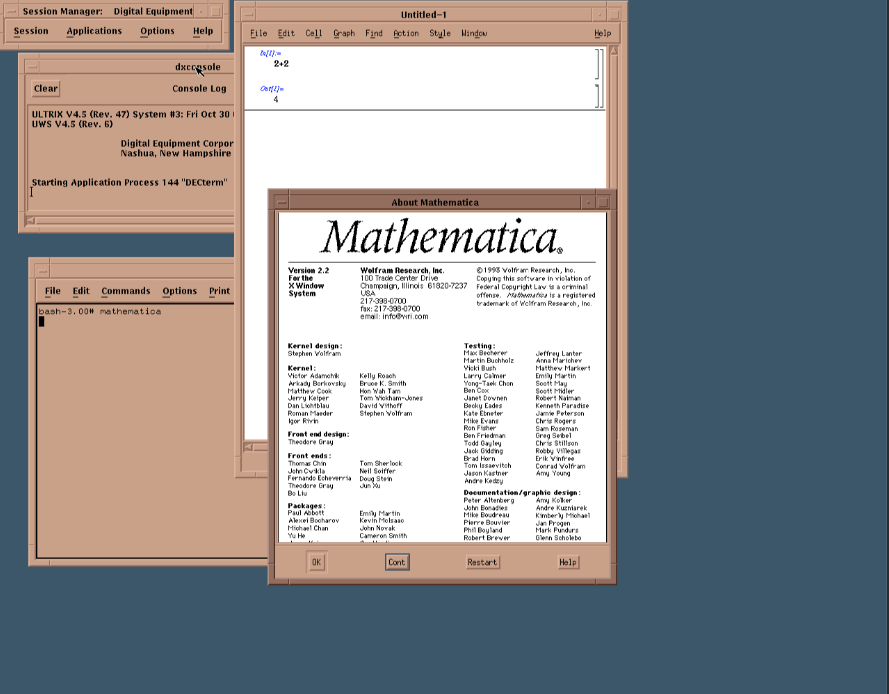
\includegraphics[scale=0.5]{nest/samplefig2.png}
			\caption{Basic elements of a communication system \cite{pahl2016interference}}
			\label{fig:samplefig2}
		\end{adjustwidth}
	\end{figure}
	
	Figure~\ref{fig:samplefig2} \lipsum[8-9] 
	
	
%
%	\bibliographystyle{IEEEtran}
%	\bibliography{references_TEMPL8}
%\end{document}
